\section{System Level Design}

\paragraph{}
In order to accomplish all of the tasks necessary for this DAQ, there were several design choices that were made at the system level.
These include decisions about what microcontroller was being used, the type of data that is being stored, the media device that data is being stored on, how other sensor or control nodes will communicate with the DAQ, what on-board sensors are on the DAQ, how or if the DAQ is able to communicate wirelessly, how a user can interface with the DAQ, and how firmware updates can be applied.

\paragraph{}
The first thing considered was how nodes are able to communicate with the DAQ.
The previous solution used CAN communicating at 1 Mbps to collect data from all nodes on the car.
This became a throughput bottleneck as lower priority CAN ids would occasionally be blocked by the high throughput, higher prioirty data.
The robustness of the CAN bus was very nice and allowed for reliable communication between all nodes on the car.
To keep the robustness of CAN and to improve issues related to throughput, CAN FD with an arbitration rate of 1 Mbps and a data rate of 5 Mbps was selected.

\paragraph{}
The next consideration was how data is stored on the DAQ.
The previous DAQ solution utilized the on-board micro SD card reader on the Teensy 3.5 and Teensy 4.1 microcontrollers and stored data in a CSV format.
The mirco SD card worked well with the small form factor, wide amount of resources available, common communication support with SPI or SDIO, and a sufficient amount of storage for 10 hours of data collection.
An alternative option would be to use an SSD.
This would allow for larger storage volumes at the cost of implementation complexity, increased mass, increased physical volume, and increased power consumption.
As a result, a micro SD card was selected as the storage media.

\paragraph{}
With an SD card as the storage media, the maximum amount of data stored is the largest constraint.
In a CSV file, each digit of a number is represented as a character, meaning that in order to represent the number 100, three bytes are required in addition to the comma deliniator.
This same number can be represented with just a single byte if the data is stored in a binary format.
Knowing that the total amount of data stored is ADD CALC RESULT HERE at 400 Hz, and the worst case values for 1 byte values being three characters, 2 byte values being 5 characters, and 4 byte numbers being ten characters, the amount of data stored over a 10 hour period would be X.
As a result, the data is stored in a binary format described in INSERT FIGURE.

\paragraph{}
To be able to parse this data, the data contained in the file is outlined at the beginning of the file, including information about data group ids, the number of variables per id, the size of each variable, and the name of the data associated with each variable as described in INSERT FIGURE.
This header is generated dynamically at runtime, so that if new data is added to the list of logged values, DAQ firmware does not need to be modified to accomondate new data.
Each data group is defined by the CAN message that will transmit the data.
Due to this, each data group is a maximum of 64 bytes in size.

\paragraph{}
The selected microcontroller was the STM32H750VBT6 from ST \cite{STMProductPage}.
This microcontroller was selected for several reasons, including a vehicle wide platform switch to STM32 microcontrollers, internal CAN FD controllers, SDIO connectivity, and a 480 MHz core frequency.
The platform switch is driven by three main criteria:
\begin{itemize}
	\item The ability to layout the chip on a PCB
	\item Having access to the debug pins for programming and debugging
	\item Large amounts of community support and open-source libraries
\end{itemize}
Teensy development boards utilize NXP chips that have most of the same features as STM32 chips, but it has slightly less community support.
Additionally, STM32 microcontrollers are used in EE 329 and CPE 316, providing experience on the platform for students who have taken those courses.

\paragraph{}
Something that all off the shelf data loggers do is provide the ability to directly connect some analog or digital sensors directly to the logger.
This functionality is desireable as it allows for a sensor to be added without external electronics, so long as sensor output is supported by the logger.
To include similar functionality, 4 analog sensor channels are available to be directly plugged into the DAQ.
This includes a 5V source for each and a GND for each.
Additionally, there is an on-board IMU and GPS to be used for the common measurements of acceleration and velocity.
These sensors are on the PCB itself and require no additional wiring by a user.

\paragraph{}
The final major piece of functionality provided by the DAQ is the ability to wirelessly transmit data acorss a range of up to 2 miles.
This is to provide live diagnostics during testing or competition to the crew it the pits to help diagnose issues and reduce time debugging if issues occur.
To do this, a radio module was added.
In order to comply with FCC and competition regulations, the main options for frequency ranges were 900 MHz, 2.4 GHz, and 5 GHz.
Since competition and testing sites are often hilly and full of trees, higher frequency nodes struggle to transmit over long distances reliably.
This drove the desire to utilize a 900 MHz radio module.
The XBee 3 Pro was selected due to its wide community support and ease of integration.
\Cref{fig:SysDiagram} describes the basic way in which these components all interface together.

\begin{figure}[H]
	\centering
	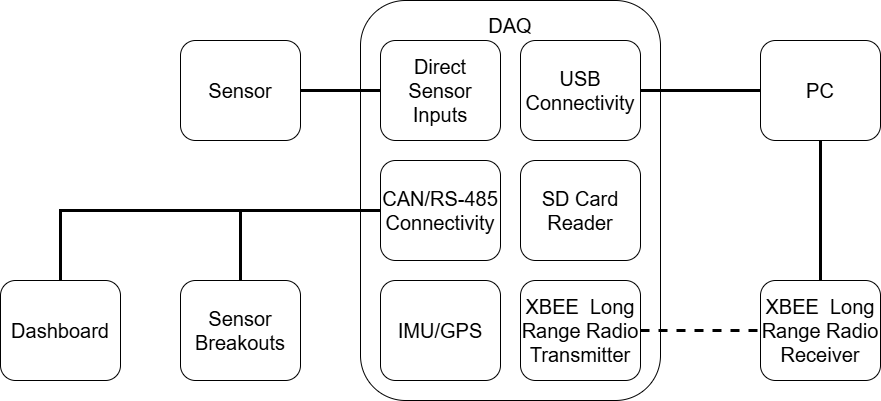
\includegraphics[width=\linewidth]{SystemDiagram.png}
	\caption{System Level Block Diagram}
	\label{fig:SysDiagram}
\end{figure}